\section{Design of UPRESSO}
\label{sec:UPRESSO}
In this section, we first present the design principle of UPRESSO with the main process phases. Then, we describe system initialization and initial registration of RP, followed by the description of algorithms for calculating the RP identifier transformation, user identifier and account. The detailed processing for each user's login is provided corresponding to the main process phases. Finally, we discuss the compatibility of UPRESSO with OIDC.

\subsection{Design Overview}
\label{subsec:overview}

%As analyzed in Section~\ref{subsec:solutions}, UPRESSO needs to provide trapdoor identification, transformed binding and user-centric confidentiality, to achieve the privacy-preserving identification, binding and confidentiality, while, the integrity is provided based on the signature inherited from existing SSO systems.
%to comfort the privacy-preserving requirements of SSO systems, UPRESSO has to allow only the exact RP to derive the user's unchanged account with a trapdoor, bind the proof with a transformation of RP’s identifier, and achieve user-centric confidentiality of the identity proof.
In Section~\ref{subsec:solutions}, we highlight three design features of UPRESSO, namely trapdoor identification, transformed binding and user-centric confidentiality, to develop a secure and privacy-preserving SSO.
Next, we will discuss three design goals that directly support these features, and explain how each goal is achieved correspondingly along the authentication flow of UPRESSO, as shown in Figure~\ref{fig:UPRESSO}.
%further divide these three requirements into three goals and
%achieve these three requirements (goals) using five phases as described in Figure~\ref{fig:UPRESSO}.
To ease the presentation, we list the notations used in this paper in Table~\ref{tbl:notations}.

\vspace{1mm}\noindent {\bf User-centric confidentiality:} {\em Generating an unforgeable and self-verifiable information for each RP to provide correct information for user-centric checking.}

In UPRESSO, such information is contained in the RP certificate ($Cert_{RP}$), which is issued by the IdP in the \emph{RP initial registration} phase (Steps a and b in Figure~\ref{fig:UPRESSO}). In each login process, the user compares the information about the RP extracted from the RP certificate and the identity proof and verifies that the identity proof issued by the IdP is generated for the requesting RP.

\vspace{1mm}\noindent {\bf Transformed binding:} {\em Generating a unique, session-specific and privacy-preserving RP identifier for the IdP to bind the identity proof to it.}

In UPRESSO, this privacy-preserving RP identifier (denoted as $PID_{RP}$) is generated from the original identifier of the RP (denoted as $ID_{RP}$) through a transformation negotiated between a pair of cooperating RP and user in the \emph{RP identifier transforming} phase (Step 2.1 in Figure~\ref{fig:UPRESSO}). As a result, non-colluding adversaries cannot view or forge this identifier, nor tamper or control its generation. Meanwhile, UPRESSO requires IdP to check the uniqueness of every $PID_{RP}$ it receives in the \emph{dynamic registration} phase (Step 2.2 in Figure~\ref{fig:UPRESSO}), so that each identity proof is bound to one unique $PID_{RP}$.



\vspace{1mm}\noindent {\bf Trapdoor identification:} {\em Generating a unique privacy-preserving user identifier based on the original user identifier and the privacy-preserving RP identifier in a way that a same user account can be derived from multiple privacy-preserving user identifiers for the same user at same RP.}

%Providing algorithms for calculating the user's identifier ($PID_U$) in identity proof and the user's account ($Account$) at the RP, allows the RP to identify the user.
%different $PID_U$ generated for different RPs, while a unique $Account$ derived at the RP with the trapdoor.

In UPRESSO, IdP computes a unique privacy-preserving user identifier (denoted as $PID_U$) based on the original user identifier (i.e., $ID_U$) and the privacy-preserving RP identifier (i.e., $PID_{RP}$) in the \emph{$PID_U$ generation} phase (Step 4 in Figure~\ref{fig:UPRESSO}). From each $PID_U$, an RP can derive a value (denoted as $Account$) with the trapdoor, i.e., the secret parameters of the RP identifier transformation, in the \emph{$Account$ processing} phase (Step 6 in Figure~\ref{fig:UPRESSO}). $Account$ uniquely identifies the user at this RP, so that it can be used to link all $PID_U$ converted from the same $ID_U$. It is worth noting that $Account$ is different from $ID_U$ and it provides no clue to derive $ID_U$, therefore, the RP still does not know the real user associated with the identity proof. Moreover, to collusive RPs, the $PID_U$s for a same user are seemingly irrelevant to each other, since they are associated with different $Account$s at these RPs.



\begin{table*}[tb]
    \caption{The notations used in UPRESSO.}
    \centering
    \begin{tabular}{|c|c|c|}
    \hline
    {Notation} & {Definition} & {} \\
    \hline
    {$p$} & {A large prime.} & {System-unique} \\
    \hline
    {$g$} & {A primitive root  modulo $p$. } & {System-unique} \\
    \hline
    {$Cert_{RP}$} & {An RP certificate. } & {RP-unique} \\
    \hline
    {$SK_{Cert}$, $PK_{Cert}$} & {The private/public key to sign/verify $Cert_{RP}$. } & {System-unique} \\
    \hline
    {$SK_{ID}$, $PK_{ID}$} & {The private/public key to sign/verify identity proof.} & {System-unique} \\
    \hline
    {$ID_U$} & {User's unique identifier at IdP.} & {System-unique} \\
    \hline
    {$PID_U$} & {User's privacy-preserving id in the identity proof.} & {One-time}\\
    \hline
    {$Account$} & {User's identifier at an RP.} & {One-time} \\
    \hline
    {$ID_{RP}$} & {RP's original identifier.} & {System-unique} \\
    \hline
    {$PID_{RP}$} & {The privacy-preserving $ID_{RP}$ transformation.} & {One-time} \\
    \hline
    {$n_U$} & {User-generated random nonce for $PID_{RP}$.} & {One-time} \\
    \hline
    {$n_{RP}$} & {RP-generated random nonce for $PID_{RP}$.} & {One-time} \\
    \hline
    {$Y_{RP}$} & {Public value for $n_{RP}$, $(ID_{RP})^{n_{RP}} \ mod p$.} & {One-time} \\
    \hline
    {$t$} & {A trapdoor, $t=(n_U*n_{RP})^{-1} mod \ (p-1)$.} & {One-time} \\
    \hline
    \end{tabular}
    \label{tbl:notations}
\end{table*}

\subsection{System Initialization and RP Initial Registration}

%In UPRESSO, a system initialization is performed to initialize the IdP, which generates $g$, $p$, $PK_{Cert}$, $SK_{Cert}$, $PK_{ID}$ and $SK_{ID}$,
%and provides  $g$, $p$, $PK_{Cert}$ and $PK_{ID}$ as the public parameters.
%Only one initial registration is performed by each RP to apply  $Cert_{RP}$ and $ID_{RP}$ from IdP.
%%the IdP needs to be initialized during at its setup, to generate the public parameters for the users and RPs.
%%The RP has to perform only one initial registration at the RP setup.
%The user triggers Steps 1-7 in Figure~\ref{fig:UPRESSO} for each login at a RP.
%%IdP setup is performed at the very beginning of UPRESSO, and will be invoked by the IdP to update the leaked $SK_{Cert}$ or $SK_{ID}$, while $g$ and $p$ will never be modified.
%%UPRESSO does not support multiple initial registrations for one RP, as the RP does not know the $ID_U$ nor the discrete logarithm of $ID_{RP}$ and fails to derive the user's new account from the old one under the Discrete Logarithm problem.

In UPRESSO, a system initialization is performed to initialize the IdP only once at the very beginning of system construction and generates the strong prime $p$, the primitive root $g$, and the key pairs ($PK_{Cert}$, $SK_{Cert}$, $PK_{ID}$ and $SK_{ID}$) for RP certificate and identity proof generation. The initial registration is performed by RP to apply $Cert_{RP}$ (for user to verify the attributes of RP) and $ID_{RP}$ (for the transformation of $ID_{RP}$) from IdP only when the new RP is built.
Besides, only the user login process are conducted in each login flow, containing the transformation ($PID_{RP}$) negotiation, the dynamic registration and the modified OIDC implicit flow.

\vspace{1mm}\noindent \textbf{System initialization.} The IdP generates two random asymmetric key pairs, ($PK_{ID}$, $SK_{ID}$) and ($PK_{Cert}$, $SK_{Cert}$),
for calculating the signatures in the identity proof and $Cert_{RP}$, respectively;
and provides $PK_{ID}$ and $PK_{Cert}$ as the public parameters for the verification of identity proof and $Cert_{RP}$.
Moreover, IdP generates a strong prime $p$, calculates  a primitive root ($g$), and provides $p$ and $g$ as the public parameters.
For $p$, we firstly randomly choose a large prime $q$, and accept  $2q+1$ as $p$ if $2q+1$ is a prime.
The strong prime $p$ makes it easier to choose $n_{u}$ and $n_{RP}$ at the user and RP for the RP identifier transformation (detailed in  Section~\ref{subsec:identifier-generation}). %With $g$, we obtain all the integers less than $p$, by calculating $g^i mod \ P$ for $0 \leq i \leq (P-1)$.
Once $SK_{Cert}$ or $SK_{ID}$ leaked, IdP may update these two asymmetric key pairs.
However, $g$ and $p$ will never be modified, otherwise, the RPs fail to link the user's accounts between two different $p$ (or $g$).
%The IdP setup and following RP initial registration are based on the features of primitive root.


\vspace{1mm}\noindent\textbf{RP initial registration.}
The RP invokes an initial registration to apply a valid and self-verifying $Cert_{RP}$ from IdP (\textbf{Goal 1}),
% as provided in Figure~\ref{fig:registration}
 which contains three steps:

\begin{enumerate}
\item RP sends IdP a $Cert_{RP}$ request $Req_{Cert_{RP}}$, which contains the distinguished name $Name_{RP}$ (e.g., DNS name) and the endpoint to receive the identity proof.
\item IdP calculates $ID_{RP} = g^r mod \ p$ with a random chosen $r$ which is coprime to $p-1$ and different from the ones for other RPs,  generates the signature ($Sig_{SK_{Cert}}$) of [$ID_{RP}, Name_{RP}$] with $SK_{Cert}$, and returns [$ID_{RP}, Name_{RP}, Sig_{SK_{Cert}}$] as $Cert_{RP}$.
\item IdP sends $Cert_{RP}$ to the RP who verifies $Cert_{RP}$ using $PK_{Cert}$.
\end{enumerate}



%1. r which is coprime to $P-1$来保证$ID_{RP}$是一个本原根,从而保证adversary无法从PID中获取ID_U, ---
%2. $ID_{RP}$不能相同,保证RP无法进行identity linkage。 ---RP可以借助类似CT的方案来保证, 没有两个合法证书被颁发给同一个ID_{RP}
To satisfy RP fails to derive $ID_U$ from $Account$ and the $Accounts$ of a user are different among RPs in \textbf{Goal 3}, two requirements on $r$ are needed  in $ID_{RP}$ generation:
\begin{itemize}
  \item $r$ should be coprime to $p-1$. This makes $ID_{RP}$ also be  a primitive root, and then prevents the RP from inferring $ID_U$ from $Account$, which is  ensured by the discrete logarithm problem.

  \item  $r$ should be different for different RPs. Otherwise, the RPs assigned the same $r$ (i.e., $ID_{RP}$), will derive the same $Account$ for a user, resulting in identity linkage. % possible.
\end{itemize}





\subsection{RP Identifier Transformation and Account Calculation}
\label{subsec:identifier-generation}
In this section, we provide the algorithms for  calculating  $PID_{RP}$, $PID_U$ and $Account$,
which are the foundations to process each user's login. %  described in Section~\ref{sebsec:loginprocess}.

\noindent\textbf{$PID_{RP}$}. Similar to Diffie-Hellman key exchange\cite{DiffieH76}, the RP and user negotiate the  $PID_{RP}$ as follows:
\begin{itemize}
  \item RP chooses a random odd number $n_{RP}$, and sends $Y_{RP} = {ID_{RP}}^{n_{RP}} mod \ p$ to the user.
  \item The user replies a random chosen odd number $n_{u}$ to the RP, and calculates $PID_{RP} = {Y_{RP}}^{n_{u}} mod \ p$.
  \item RP also derives $PID_{RP}$ with the received $n_{u}$.
\end{itemize}

As denoted in Equation~\ref{equ:RPIDT}, ${ID_{RP}}$ cannot be derived from $PID_{RP}$, which satisfies IdP never infers ${ID_{RP}}$ from $PID_{RP}$ in \textbf{Goal 2}.
%Therefore, $PID_{RP}$ is denoted as Equation~\ref{equ:ID_{RP}T}. The IdP fails to infer ${ID_{RP}}$ from $PID_{RP}$ (\textbf{Privacy in Goal 2}).
   \begin{equation}
   PID_{RP} = {Y_{RP}}^{n_{u}} = {ID_{RP}}^{n_{u}* n_{RP}} mod \ p
   \label{equ:ID_{RP}T}
   \end{equation}

To ensure $PID_{RP}$ not controlled by the adversary in \textbf{Goal 2},
 $PID_{RP}$ should not be determined by  either the RP or user. %, as the adversary may control either the RP or user.
Otherwise, malicious users may make the victim RP accept an identity proof issued for another RP; or collusive RPs may provide the correlated $PID_{RP}$ for potential identity linkage.
%The generation ensures that $PID_{RP}$ cannot be determined by neither (malicious) user nor RP, which prevents the adversary from constructing a identity proof to be accepted by two or more RPs (\textbf{Security in Goal 2}).
In UPRESSO, RP fails to control the $PID_{RP}$ generation, as it provides $Y_{RP}$ before obtaining $n_{u}$ and the modification of $Y_{RP}$ will trigger the user to generate another different  $n_{u}$. The Discrete Logarithm problem prevents the user from choosing an $n_{u}$ for a specified $PID_{RP}$ on the received $Y_{RP}$.

In UPRESSO, both $n_{RP}$ and $n_{u}$ are odd numbers, therefore $n_{RP}*n_{u}$ is an odd number and coprime to the even $p-1$, which ensures that the inverse $(n_{RP}*n_{u})^{-1}$ always exists, where  $(n_{RP}*n_{u})^{-1} * (n_{RP}*n_{u}) = 1 \ mod \ (p-1)$. The inverse  serves as  the trapdoor $t$ for $Accout$, which makes:
\begin{equation}
(PID_{RP})^t = ID_{RP} \ mod \ p
\label{equ:trapdoor}
\end{equation}


\noindent\textbf{$PID_U$}. The IdP generates the $PID_U$ based on the user's $ID_U$ and the user-provided $PID_{RP}$, as denoted in Equation~\ref{equ:PID_U}.
The corporative generation of $PID_{RP}$, ensures unrelated $PID_U$  for different RPs in \textbf{Goal 3}. Also, RP fails to derive $ID_U$ from either $PID_U$ in \textbf{Goal 3}, as
   $PID_{RP}$ is a primite root modulo $p$, and the $ID_U$ cannot be derived from $PID_{RP}^{ID_U}$.
\begin{equation}
 PID_U = {PID_{RP}}^{ID_U} \ mod \ p
 \label{equ:PID_U}
\end{equation}

Finally, the RP calculates $PID_U^t mod \ p$ as the  user's account, where $PID_U$ is received from the user and $t$ is derived in the generation of $PID_{RP}$. Equation~\ref{equ:account} demonstrates that $Account$ is unchanged to the RP during a user's multiple logins, satisfying RP derives the user's unique $Account$  from $PID_U$ with the  trapdoor and  RP fails to derive $ID_U$ from either $Account$ in \textbf{Goal 3}. The different $ID_{RP}$ ensures the $Accounts$ of a user are different among RPs in \textbf{Goal 3}.

 \begin{equation}
   Account = ({PID_{RP}}^{ID_U})^t = {ID_{RP}}^{ID_U} mod \ p
   \label{equ:account}
   \end{equation}


\subsection{User Login}
\label{sebsec:loginprocess}
In this section, we present the detailed process for each user's login as shown in Figure~\ref{fig:process}. %The process corresponds to the goals 2-5 defined in Section~\ref{subsec:overview}.

\begin{figure*}
  \centering
  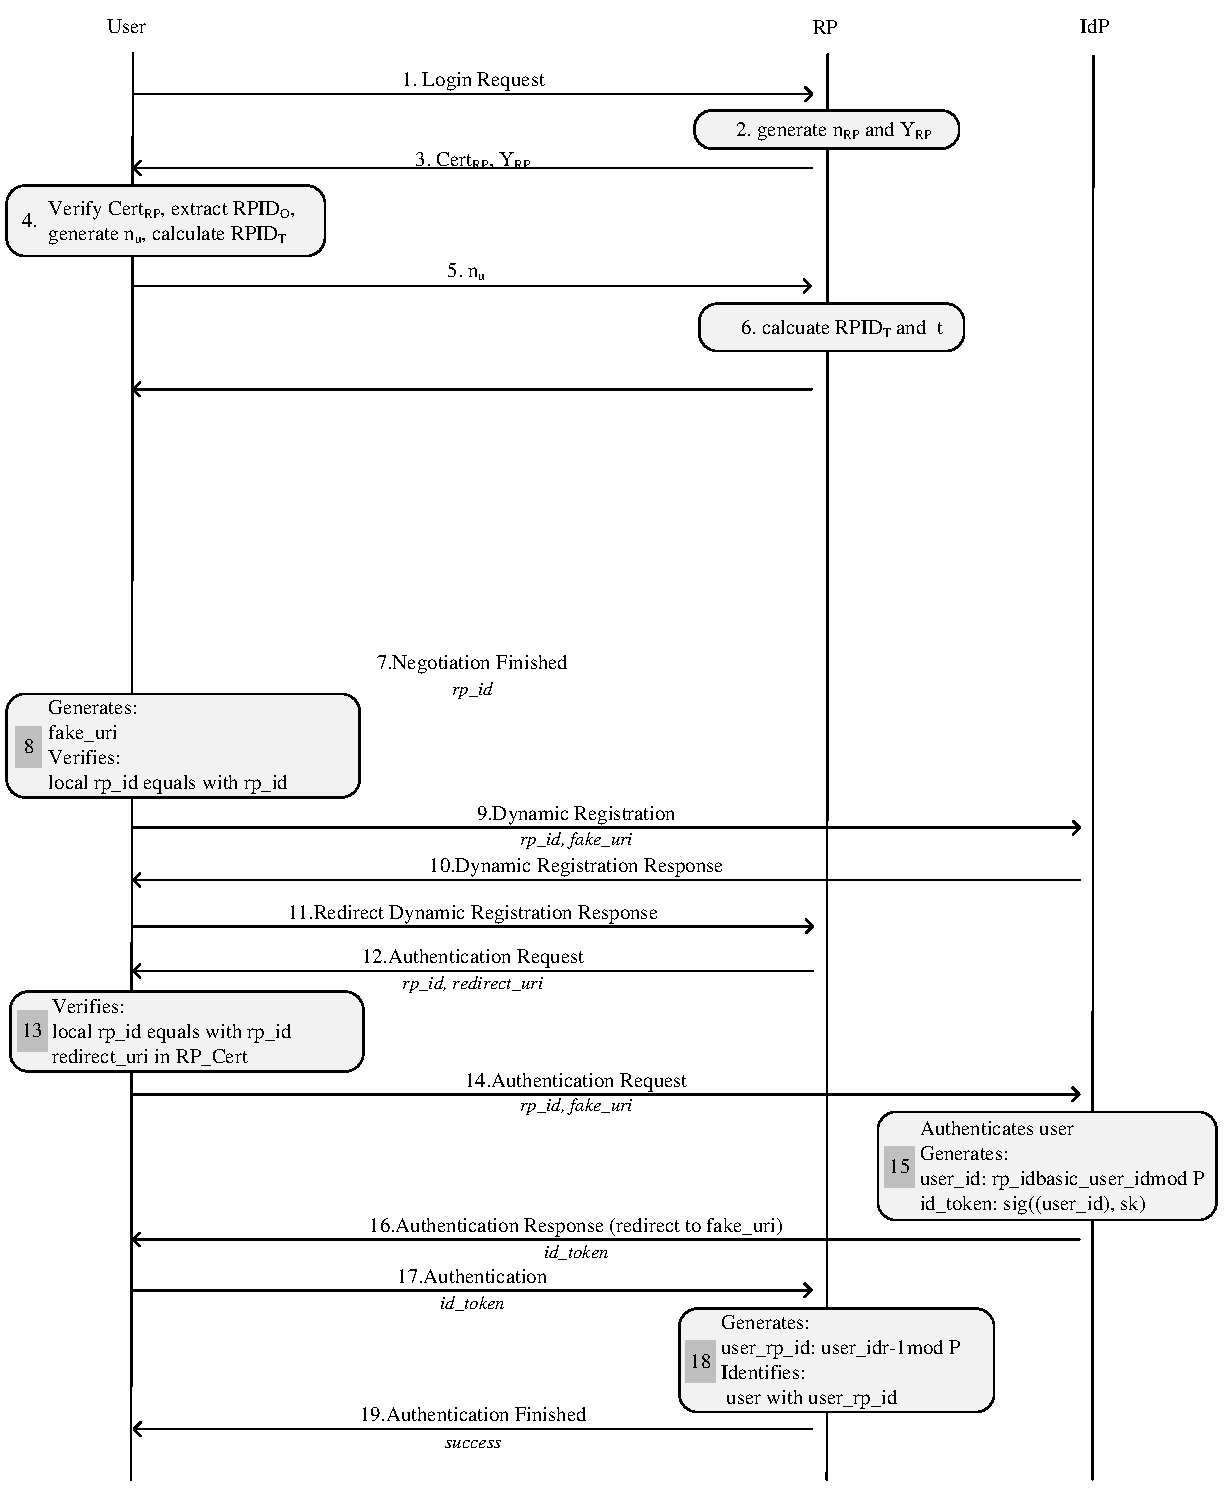
\includegraphics[width=0.85\linewidth]{fig/process.pdf}
  \caption{Process for each user login.}
  \label{fig:process}
\end{figure*}

In RP identifer transforming phase, the user and RP corporately process as follows. \textbf{(1)} The user sends a login request to trigger the negotiation of $PID_{RP}$. \textbf{(2)} RP chooses the random $n_{RP}$, and calculates $Y_{RP}$ as described in Section~\ref{subsec:identifier-generation}. \textbf{(3)} RP sends $Cert_{RP}$ with $Y_{RP}$ to the user.  \textbf{(4)} The user halts the login process if the provided $Cert_{RP}$ is invalid; otherwise, it extracts $ID_{RP}$ from $Cert_{RP}$, and calculates $PID_{RP}$ with a random chosen $n_U$ as in Section~\ref{subsec:identifier-generation}. \textbf{(5)} The user sends $n_U$ and $PID_{RP}$ to the RP. \textbf{(6)} RP calculates $PID_{RP}$ using the received $n_U$ with $Y_{RP}$ as in Section~\ref{subsec:identifier-generation}, and rejects the user's login request if the calculated $PID_{RP}$ is inconsistent with the received one. After that, RP derives the trapdoor $t$ as in Section~\ref{subsec:identifier-generation}, which will be used in calculating $Account$. \textbf{(7)} RP sends the calculated $PID_{RP}$ to the user, who will halt the login if the received $PID_{RP}$ is different from the cached one.

In the dynamic registration phase, the user registers the newly generated $PID_{RP}$ at the IdP as follows. \textbf{(8)} The user generates an one-time endpoint (used in Section~\ref{subsec:compatible}) if the received $PID_{RP}$ is accepted. \textbf{(9)} Then, the user registers the RP with the $PID_{RP}$ and one-time endpoint. \textbf{(10)} If $PID_{RP}$ is globally unique and is a primitive root module $p$, IdP sets the flag $RegRes$ as $OK$ (otherwise $FAIL$), and constructs the reply in the form of
[$RegRes$, $RegMes$, $Sig_{SK_{ID}}$]
%[$RegRes$, $timestamp$, $PID_{RP}$, $Sig_{SK_ID}$] where $timestamp$ is the time generating this reply and
where $RegMes$ is the response to traditional dynamic registration containing $PID_{RP}$, issuing time as well as other attributes and $Sig_{SK_{ID}}$ is the signature of the other elements using the private key $SK_{ID}$ (ensuring unique $PID_{RP}$ for binding in \textbf{Goal 2}). \textbf{(11)} The user forwards the registration result to the RP. The user obtains $RegRes$ directly as the connection between the user and IdP is secure, while the RP accepts the $RegRes$ only when $Sig_{SK_{ID}}$ is valid
%, $timestamp$ is correct and $PID_{RP}$ is the same as the cached one.
and $RegMes$ is issued for the $PID_{RP}$ within the valid period. The user and RP will negotiate a new $PID_{RP}$ if $RegRes$ is $FAIL$.

To acquire the $PID_U$, the user corporates with the RP and IdP as follows. \textbf{(12)} RP constructs an identity proof request with the correctly registered $PID_{RP}$ and the endpoint (the form of the request is detailed in Section~\ref{subsec:compatible}). \textbf{(13)} The user halts the login process if the received $PID_{RP}$ is different from the previous one. \textbf{(14)} The user replaces the endpoint with the registered one-time endpoint, and sends it with the identity proof request to the IdP. \textbf{(15)} IdP requires the user to provide the correct credentials if the user hasn't been unauthenticated; and rejects the request if the binding of $PID_{RP}$ and the one-time endpoint doesn't exist in the registered ones. Then, IdP generates the $PID_U$ as in Section~\ref{subsec:identifier-generation}, and constructs the identity proof with $PID_{RP}$, $PID_U$, the valid period, issuing time and other attribute values, by attaching a signature of these elements using the private key $SK_{ID}$. \textbf{(16)} IdP sends the identity proof with the one-time endpoint to the user. \textbf{(17)} The user forwards the identity proof to the RP's endpoint corresponding to the one-time endpoint.

Finally, RP derives the user's  $Account$ from $PID_U$ as follows. \textbf{(18)} RP accepts the identity proof only when the signature is correctly verified with $PK_{ID}$, $PID_{RP}$ is the same as the negotiated one, the issuing time is less than current time, and the current time is in the validity period. If the identity proof is incorrect, RP returns login fail to the user who will trigger another login request. Otherwise, RP calculates the $Account$ as in Section~\ref{subsec:identifier-generation}. \textbf{(19)} RP sends the login result to the user and begins to provide the personalized service.


\subsection{Compatibility with OIDC}
\label{subsec:compatible}
UPRESSO is compatible with the implicit protocol flow of OIDC (authorization code flow is discussed in Section~\ref{sec:discussion}).

In UPRESSO, the formats of identity proof request and identity proof are the same as the ones in OIDC. In details, each element of the identity proof request in OIDC is contained in UPRESSO as follows: the RP's identifier ($PID_{RP}$ in UPRESSO), the endpoint (one-time endpoint in the request from the user in UPRESSO) and the set of required attributes (also supported by UPRESSO but not listed here). The identity proof in UPRESSO is also exactly the same as the one in OIDC, which includes RP's identifer ($PID_{RP}$ in UPRESSO), the user's PPID ($PID_U$ in UPRESSO), the issuer, validity period, issuing time, other requested attributes and a signature generated by $SK_{ID}$. % the IdP's private key.

The same formats of identity proof request and identity proof make the verification same in OIDC and UPRESSO. The IdP, in both UPRESSO and OIDC, verifies the identity proof request, by checking whether the mapping of RP's identifier and endpoint exists in the registered ones. The RP, in both UPRESSO and OIDC, verifies the identity proof, by checking the signature, the consistency of RP's identifer in the identity proof and the one it owns, the validity period, issuing time and the freshness (which is checked based on a nonce in  OIDC, while  $PID_{RP}$ serves as the nonce in UPRESSO).

The RP's extra processes needed in UPRESSO may be achieved using the existing interfaces defined in OIDC.
UPRESSO requires that $PID_{RP}$ is globally unique, which can be achieved through the dynamic registration (described in Section~\ref{sec:background}) provided by IdP in OIDC.
In UPRESSO, the dynamic registration is invoked by the user instead of the RP to prevent the curious IdP linking  the dynamic registration from RP with the identity proof request sent by the user.
To avoid the IdP to infer the RP's identity through the registration token in dynamic registration,
a common  registration token is used in UPRESSO.
As the registration response is transmitted through the user instead of server-to-server transmission between RP and IdP, the extra signature is required to guarantee the integrity of response. Moreover, the endpoint in the dynamic registration request is replaced with an one-time endpoint, to avoid the RP's identifying information to be leaked to the IdP.


The modification of the RP required by UPRESSO may be achieved only using the existing interfaces provided by the current implementations of OIDC.
Based on the software development kit (SDK) in existing OIDC implementations for RP, the Steps 2-3, 5-7, 12 (in Figure~\ref{fig:process}) in RP may be integrated in the interface for constructing identity proof request;
Step 18 in Figure~\ref{fig:process} may be combined with the interface for  parsing identity proof.

The processes at the user may be achieved through an extension at the user agent,
which captures the identity proof (and request)  without modifying existing message transmission at the IdP and RP (i.e., redirection mechanism). % as described in Section~\ref{sec:implementation}.


Only the RP initial registration, step 10 and Step 15 in Figure~\ref{fig:process} require the modification at IdP.

In the actually deployed systems, the comprehensive update of RPs would be the long term procedure, during which there might be the updated and legacy RPs at the same time. In USPRESSO, the legacy OIDC flow started by the legacy user agent (starting the login by clicking the button in the RP's web page) is supported as it only requires the step 1, 12, 14, 15, 16 and 17 in Figure~\ref{fig:process} and the process is accepted by the IdP and legacy user agent, only requiring the IdP to tag the legacy $ID_{RP}$ and provide the legacy PPID to these $ID_{RP}$.

